%%%%%%%%%%%%%%%%%%%%%%%%%%%%% Define Exam %%%%%%%%%%%%%%%%%%%%%%%%%%%%%%%%%%
\documentclass[addpoints]{exam}
%%%%%%%%%%%%%%%%%%%%%%%%%%%%%%%%%%%%%%%%%%%%%%%%%%%%%%%%%%%%%%%%%%%%%%%%%%%%%%%

%%%%%%%%%%%%%%%%%%%%%%%%%%%%% Using Packages %%%%%%%%%%%%%%%%%%%%%%%%%%%%%%%%%%
\usepackage{amsmath, amssymb, amsthm, amsfonts, geometry, venndiagram, tikz}
\usepackage{graphicx, xcolor, color, wrapfig, parskip, float, tabularx}
\usepackage[breaklinks]{hyperref}
\usepackage{colortbl, caption}
\usepackage{listings, mdframed, subfig, matlab-prettifier, hyperref, pythonhighlight}
\usepackage{lipsum, bookmark, booktabs, empheq, titlesec, verbatim, subfig, pdfpages, comment, subfloat}

%%%%%%%%%%%%%%%%%%%%%%%%%%%%%%%%%%%%%%%%%%%%%%%%%%%%%%%%%%%%%%%%%%%%%%%%%%%%%%%
\definecolor{codebackground}{rgb}{0.95,0.95,0.95}
\definecolor{codegray}{rgb}{0.5,0.5,0.5}
\definecolor{codepurple}{rgb}{0.58,0,0.82}
\definecolor{codeblue}{rgb}{0.13,0.29,0.53}
\definecolor{ocre}{RGB}{243,102,25}
\definecolor{mygray}{RGB}{243,243,244}
\definecolor{deepGreen}{RGB}{26,111,0}
\definecolor{shallowGreen}{RGB}{235,255,255}
\definecolor{deepBlue}{RGB}{61,124,222}
\definecolor{shallowBlue}{RGB}{235,249,255}
\definecolor{softgray}{rgb}{0.95, 0.95, 0.95}
\definecolor{codegreen}{rgb}{0,0.6,0}
\definecolor{codegray}{rgb}{0.5,0.5,0.5}
\definecolor{codepurple}{rgb}{0.58,0,0.82}
\definecolor{backcolour}{rgb}{0.95,0.95,0.92}

%Code listing style named "mystyle"
\lstdefinestyle{mystyle}{
  backgroundcolor=\color{backcolour}, commentstyle=\color{codegreen},
  keywordstyle=\color{magenta},
  numberstyle=\tiny\color{codegray},
  stringstyle=\color{codepurple},
  basicstyle=\ttfamily\footnotesize,
  breakatwhitespace=false,         
  breaklines=true,                 
  captionpos=b,                    
  keepspaces=true,                 
  numbers=left,                    
  numbersep=5pt,                  
  showspaces=false,                
  showstringspaces=false,
  showtabs=false,                  
  tabsize=2
}

%"mystyle" code listing set
\lstset{style=mystyle}

\usetikzlibrary{arrows,shapes,positioning,shadows,trees, backgrounds}

\tikzstyle{arrow} = [->,>=stealth]
\tikzstyle{node} = [auto,font=\footnotesize,draw,circle]

%%%%%%%%%%%%%%%%%%%%%%%%%%%%% Header and Footer %%%%%%%%%%%%%%%%%%%%%%%%%%%%%%%%%%
\pagestyle{headandfoot}
\runningheadrule
\runningfootrule
\runningheader{Algorithms: Design and Analysis}{Weekly Challenge 08}{CS 412}
\runningfooter{}{Page \thepage\ of \numpages}{}
\firstpageheader{}{}{}
%%%%%%%%%%%%%%%%%%%%%%%%%%%%%%%%%%%%%%%%%%%%%%%%%%%%%%%%%%%%%%%%%%%%%%%%%%%%%%%

% Other Settings
% \boxedpoints
\printanswers
\qformat{}  %Comment this to number questions, uncomment this to not number questions

\newcommand\union\cup
\newcommand\inter\cap

%%%%%%%%%%%%%%%%%%%%%%%%%%%%%%% Title & Author %%%%%%%%%%%%%%%%%%%%%%%%%%%%%%%%

\title{Algorithms: Design and Analysis - CS 412 \vspace*{-4mm}}
\author{Weekly Challenge 08: Dynamic Programming}
\date{\vspace*{-4mm} Ali Muhammad Asad - aa07190}

% \pgfplotsset{compat=1.18}

%%%%%%%%%%%%%%%%%%%%%%%%%%%%%%%%%%%%%%%%%%%%%%%%%%%%%%%%%%%%%%%%%%%%%%%%%%%%%%%

\begin{document}
\maketitle

\begin{questions}
    \question[1]
      We are going to implement the rod cutting algorithm from CLRS 15.1 in a file \texttt{cutrod.py}. We will implement the following three versions of the solution: \textit{top-down recursive}, \textit{top-down memoized}, and \textit{bottom-up}. Your code will be tested by \pyth{pytest} using the file, \texttt{test\_cutrod.py}, given in \texttt{WC8\_DP.zip}. To test your code implementation, open the directory containing \texttt{test\_cutrod.py} and \texttt{cutrod.py} in the terminal, and run the following command:
    \begin{lstlisting}[language=bash]
    pytest test_cutrod.py
\end{lstlisting}
      \textbf{TASKS}:
      \begin{parts}
      \part Write the top-down recursive version in a function, \pyth{cut_rod}.
      \part Write the top-down memoized version in a function, \pyth{cut_rod_memoized}.
      \part Write the bottom-up version in a function, \pyth{cut_rod_bottom_up}.
      \part All functions take two arguments, \texttt{p} and \texttt{n}, where \texttt{p} is the price array and \texttt{n} is the length of the rod. \texttt{p[i]} is the price of a rod of length \texttt{i}. All prices are positive and increase with length.
      \part Write all functions in the file, \texttt{cutrod.py}.
      \part Ensure that all tests pass by running \pyth{pytest} locally.
      \part Do not include any external packages.  
      \part You may modify the error messages in \texttt{test\_cutrod.py} to convey more information if you wish, but you may not alter any other functionality in it.
      \part Plot the running time of the three versions against \texttt{n} and include them below along with any relevant observations. Your code for plotting should be in \texttt{plot.py}. 
      \end{parts}
    
    \newpage
    \begin{solution}
			We defined the \pyth{plot.py} script as follows:
			\begin{lstlisting}[style=mystyle]
import time, matplotlib.pyplot as plt
from cutrod import *

def measure_time(func, p, n):
		start = time.time()
		func(p, n)
		end = time.time()
		return end - start

def plot_times(n_values, times, labels):
		for i in range(len(times)):
				plt.plot(n_values, times[i], label=labels[i])
		plt.xlabel('n'); plt.ylabel('time (s)'); plt.legend(); plt.show()

def main():
		n_values = list(range(1, 25))
		p = [i for i in range(1, 25)]
		functions = [cut_rod, cut_rod_memoize, cut_rod_bottom_up]
		labels = ['Recursive', 'Memoized', 'Bottom Up']
		times = []

		for func in functions:
				func_times = []
				for n in n_values:
						t = measure_time(func, p, n)
						print(f'{func.__name__}({n=}) took {t:.6f} seconds')
						func_times.append(t)
				times.append(func_times)
		
		plot_times(n_values, times, labels)

if __name__ == '__main__':
		main()
\end{lstlisting}

The above script basically measures the running time of the three functions for increasing values of $n$ and then plots the running times against $n$. The running times are measured using the \pyth{time} module in Python. The \pyth{measure_time} function takes a function, \pyth{func}, and measures the time it takes to run the function for a given \pyth{n}. The \pyth{plot_times} function takes the running times of the three functions and plots them against $n$. The \pyth{main} function then measures the running times of the three functions for increasing values of $n$ and then plots the running times against $n$.

		\newpage
			For our three functions, we got the running times as follows:
			\begin{figure}[H]
				\centering
				\begin{tabular}{| c | c |}
					\hline
					\subfloat[n = 5]{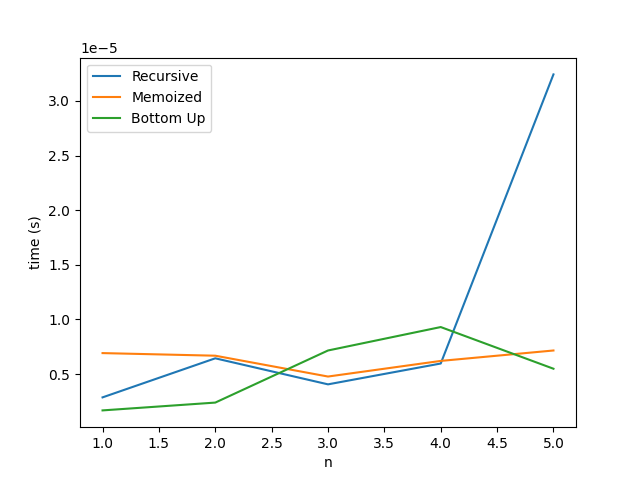
\includegraphics[width=0.45\textwidth]{results/n_5.png}} & \subfloat[n = 10]{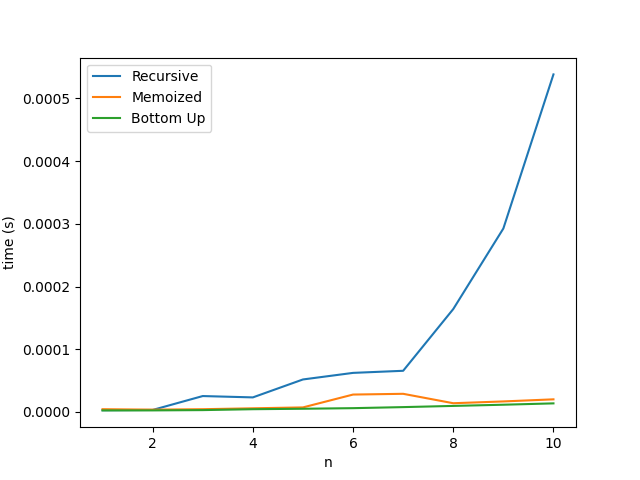
\includegraphics[width=0.45\textwidth]{results/n_10.png}} \\
					\hline
					\subfloat[n = 15]{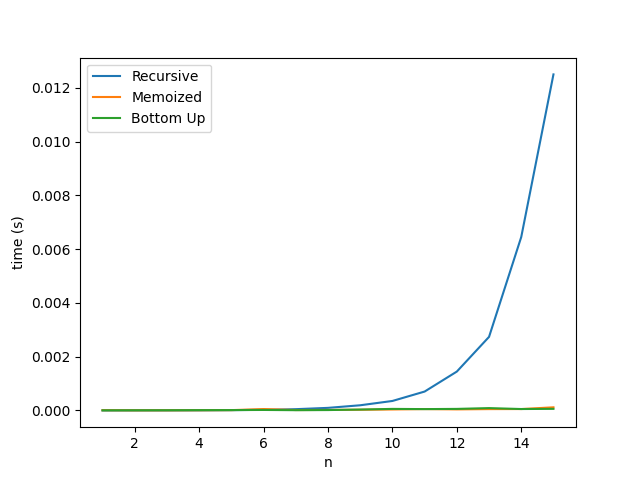
\includegraphics[width=0.45\textwidth]{results/n_15.png}} & \subfloat[n = 20]{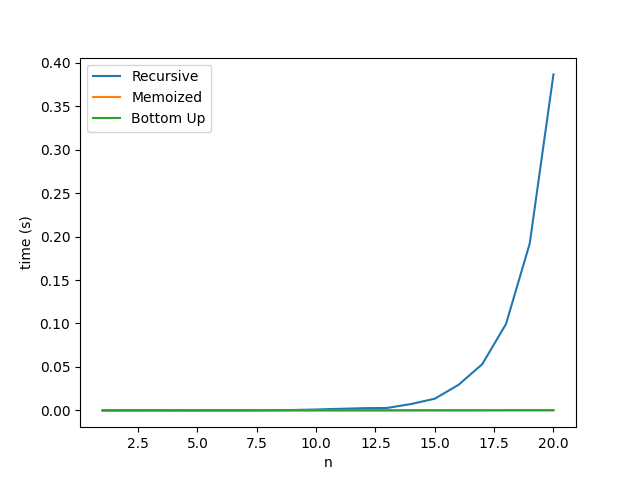
\includegraphics[width=0.45\textwidth]{results/n_20.png}} \\
					% \hline
					% \subfloat[subcaption]{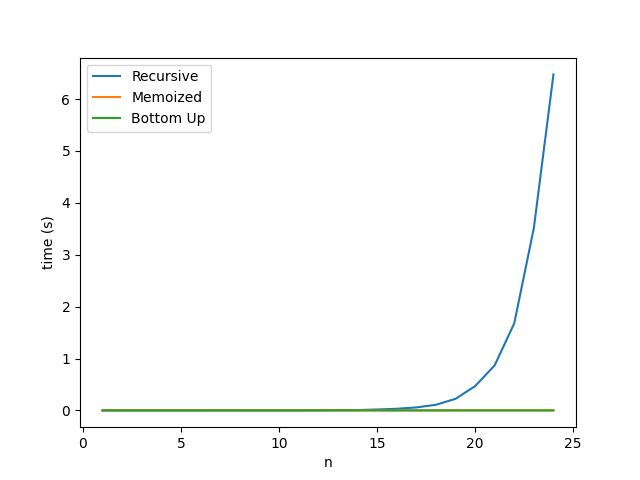
\includegraphics[width=0.475\textwidth]{n_25.png}} & \subfloat[subcaption]{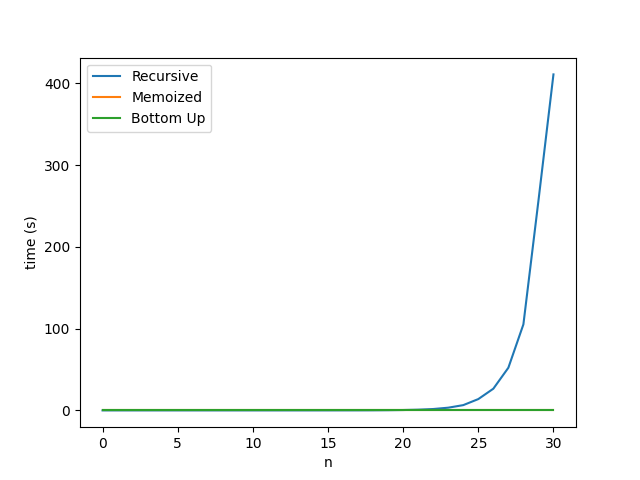
\includegraphics[width=0.475\textwidth]{n_30.png}} \\ 
					\hline
				\end{tabular}
			\end{figure}

			From the above plots for increasing values of $n$ upto 20, we can see that the running time of the recursive version is the highest, which exponentially shoots up with increasing $n$ while the memoized and bottom-up version have barely any increase in their runtimes. This is because the the recursive version recursively branches into two possiblities on each iteration from up to $n$; cut or don't cut. Then for each length from 0 to $n$, the function is exploring two possiblities - making a cut or not making a cut. This results in a binary tree where each node represents a function call, and each branch gets a decision to cut or not to cut. Then the runtime of the recursive version is $O(2^n)$, which is exponential. The memoized version, on the other hand, stores the results of the subproblems in an array and uses them to avoid recomputation of the same subproblems. This results in a polynomial time complexity of $O(n^2)$. The bottom-up version, on the other hand, iteratively computes the subproblems from the bottom up, and hence has a polynomial time complexity of $O(n^2)$ as well. Therefore, the bottom-up and memoized versions are much faster than the recursive version. (In practice, the bottom up is most often faster since it doesn't have the overhead of recursion).
    \end{solution}
\end{questions}
\end{document}